%%%%%%%%%%%%%%%%%%%%%%%%%%%%%%%%%%%
%This is the LaTeX ARTICLE template for RSC journals
%Copyright The Royal Society of Chemistry 2016
%%%%%%%%%%%%%%%%%%%%%%%%%%%%%%%%%%%

\documentclass[twoside,twocolumn,9pt]{article}
\usepackage{extsizes}
\usepackage[super,sort&compress,comma]{natbib}
\usepackage[version=3]{mhchem}
\usepackage[left=1.5cm, right=1.5cm, top=1.785cm, bottom=2.0cm]{geometry}
\usepackage{balance}
\usepackage{mathptmx}
\usepackage{sectsty}
\usepackage{graphicx}
\usepackage{lastpage}
\usepackage[format=plain,justification=justified,singlelinecheck=false,font={stretch=1.125,small,sf},labelfont=bf,labelsep=space]{caption}
\usepackage{float}
\usepackage{fancyhdr}
\usepackage{fnpos}
\usepackage[english]{babel}
\addto{\captionsenglish}{%
  \renewcommand{\refname}{Notes and references}
}
\usepackage{array}
\usepackage{droidsans}
\usepackage{charter}
\usepackage[T1]{fontenc}
\usepackage[usenames,dvipsnames]{xcolor}
\usepackage{setspace}
\usepackage[compact]{titlesec}
\usepackage{hyperref}
%%%Please don't disable any packages in the preamble, as this may cause the template to display incorrectly.%%%

\usepackage{epstopdf}%This line makes .eps figures into .pdf - please comment out if not required.

% Additional packages for this manuscript
\usepackage{amsmath,amssymb}
% mathptmx removes \myhbar; define explicitly
\newcommand{\myhbar}{\mathchar'26\mkern-9mu h}
\usepackage{booktabs}
\usepackage{siunitx}
\usepackage{multirow}

\definecolor{cream}{RGB}{222,217,201}

\begin{document}

\pagestyle{fancy}
\thispagestyle{plain}
\fancypagestyle{plain}{
%%%HEADER%%%
\renewcommand{\headrulewidth}{0pt}
}
%%%END OF HEADER%%%

%%%PAGE SETUP - Please do not change any commands within this section%%%
\makeFNbottom
\makeatletter
\renewcommand\LARGE{\@setfontsize\LARGE{15pt}{17}}
\renewcommand\Large{\@setfontsize\Large{12pt}{14}}
\renewcommand\large{\@setfontsize\large{10pt}{12}}
\renewcommand\footnotesize{\@setfontsize\footnotesize{7pt}{10}}
\makeatother

\renewcommand{\thefootnote}{\fnsymbol{footnote}}
\renewcommand\footnoterule{\vspace*{1pt}%
\color{cream}\hrule width 3.5in height 0.4pt \color{black}\vspace*{5pt}}
\setcounter{secnumdepth}{5}

\makeatletter
\renewcommand\@biblabel[1]{#1}
\renewcommand\@makefntext[1]%
{\noindent\makebox[0pt][r]{\@thefnmark\,}#1}
\makeatother
\renewcommand{\figurename}{\small{Fig.}~}
\sectionfont{\sffamily\Large}
\subsectionfont{\normalsize}
\subsubsectionfont{\bf}
\setstretch{1.125} %In particular, please do not alter this line.
\setlength{\skip\footins}{0.8cm}
\setlength{\footnotesep}{0.25cm}
\setlength{\jot}{10pt}
\titlespacing*{\section}{0pt}{4pt}{4pt}
\titlespacing*{\subsection}{0pt}{15pt}{1pt}
%%%END OF PAGE SETUP%%%

%%%FOOTER%%%
\fancyfoot{}
\fancyfoot[LO,RE]{\vspace{-7.1pt}
\includegraphics[height=9pt]{head_foot/LF}}
\fancyfoot[CO]{\vspace{-7.1pt}\hspace{13.2cm}
\includegraphics{head_foot/RF}}
\fancyfoot[CE]{\vspace{-7.2pt}\hspace{-14.2cm}
\includegraphics{head_foot/RF}}
\fancyfoot[RO]{\footnotesize{\sffamily{1--\pageref{LastPage} ~\textbar  \hspace{2pt}\thepage}}}
\fancyfoot[LE]{\footnotesize{\sffamily{\thepage~\textbar\hspace{3.45cm} 1--\pageref{LastPage}}}}
\fancyhead{}
\renewcommand{\headrulewidth}{0pt}
\renewcommand{\footrulewidth}{0pt}
\setlength{\arrayrulewidth}{1pt}
\setlength{\columnsep}{6.5mm}
\setlength\bibsep{1pt}
%%%END OF FOOTER%%%

%%%FIGURE SETUP - please do not change any commands within this section%%%
\makeatletter
\newlength{\figrulesep}
\setlength{\figrulesep}{0.5\textfloatsep}

\newcommand{\topfigrule}{\vspace*{-1pt}%
\noindent{\color{cream}\rule[-\figrulesep]{\columnwidth}{1.5pt}} }

\newcommand{\botfigrule}{\vspace*{-2pt}%
\noindent{\color{cream}\rule[\figrulesep]{\columnwidth}{1.5pt}} }

\newcommand{\dblfigrule}{\vspace*{-1pt}%
\noindent{\color{cream}\rule[-\figrulesep]{\textwidth}{1.5pt}} }

\makeatother
%%%END OF FIGURE SETUP%%%

%%%TITLE, AUTHORS AND ABSTRACT%%%
\twocolumn[
  \begin{@twocolumnfalse}
{
\includegraphics[height=30pt]{head_foot/journal_name}\hfill\raisebox{0pt}[0pt][0pt]{
\includegraphics[height=55pt]{head_foot/RSC_LOGO_CMYK}}\\[1ex]

\includegraphics[width=18.5cm]{head_foot/header_bar}}\par
\vspace{1em}
\sffamily
\begin{tabular}{m{4.5cm} p{13.5cm} }


\includegraphics{head_foot/DOI} & \noindent\LARGE{\textbf{Systematic screening of brain neurotransmitter enzymes for radical pair mechanism competence reveals quantitative constraints on magnetic field sensitivity$^\dag$}} \\%Article title
\vspace{0.3cm} & \vspace{0.3cm} \\

 & \noindent\large{Hikaru Wakaura$^{\ast}$\textit{$^{a}$}} \\%Author names
 
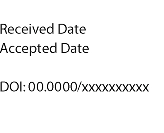
\includegraphics{head_foot/dates} & \noindent\normalsize{We screen nine phosphorus-containing brain enzymes for radical pair mechanism (RPM) competence using semi-empirical (GFN2-xTB) and \textit{ab initio} (CASSCF/NEVPT2) quantum chemistry, assigning cofactor-specific \ce{^{31}P} hyperfine couplings and computing spin relaxation under physiological conditions (50~\si{\micro\tesla}, 310~K). Eight enzymes satisfy all seven necessary spin-parameter conditions, but the dominant discriminant---\ce{^{31}P} nuclear coherence time, scaling as $r^{-6}$ via paramagnetic relaxation enhancement---creates a 64-fold gap between FAD (160~\si{\micro\second}) and PLP (2.5~\si{\micro\second}) enzymes. Density matrix simulation of an 8-spin MAO-A model gives MFE~$= -4.4\%$ at $J = 0$, but this is negligible at the crystallographic radical pair distance ($|J| \sim 500$--$1000$~MHz). CASSCF(2,2)/NEVPT2 analysis finds low diradical character ($y_0 < 0.1$), disfavouring single-electron transfer. For CRY ([\ce{FAD^{.-}\bond{...}TrpH^{.+}}], $|J| < 1$~MHz), 8-spin simulation predicts MFE~$= -5.6\%$ at $B = 0.29$~mT and $-0.55\%$ at Earth's field. Exchange coupling, mechanism, and homeostasis collectively restrict functional RPM to cryptochrome, the sole enzyme with a confirmed spatially separated radical pair.} \\%Abstract
 
\end{tabular} 

 \end{@twocolumnfalse} \vspace{0.6cm} 

  ]
%%%END OF TITLE, AUTHORS AND ABSTRACT%%%

%%%FONT SETUP - please do not change any commands within this section
\renewcommand*\rmdefault{bch}\normalfont\upshape
\rmfamily
\section*{}
\vspace{-1cm}


%%%FOOTNOTES%%%

\footnotetext{\textit{$^{a}$~QIRI (Quantum Integrated Research Institute Inc.), Tokyo 107-0061, Japan. E-mail: h.wakaura@deeptell.jp}}

\footnotetext{\dag~Electronic Supplementary Information (ESI) available: Detailed derivations of spin relaxation expressions, extended data tables, and additional computational details. See DOI: 00.0000/00000000.}


%%%END OF FOOTNOTES%%%

%%%MAIN TEXT%%%%

\section{Introduction}

Quantum biology has advanced rapidly over the past two decades, with proposed quantum effects in photosynthetic energy transfer\cite{Engel2007,Lambert2013} (though the functional role of observed coherences remains debated), established hydrogen tunnelling in enzymes,\cite{Klinman2013} and avian magnetoreception.\cite{Ritz2000,Maeda2012,Xu2021} Among these, the radical pair mechanism (RPM) stands out as the most experimentally validated: transient radical pairs generated by electron transfer undergo coherent singlet--triplet interconversion driven by hyperfine coupling (HFC) to magnetic nuclei, producing reaction yields that are sensitive to weak magnetic fields.\cite{Hore2016,Steiner1989} The RPM in cryptochrome has been confirmed to respond to Earth-strength fields,\cite{Xu2021,Kattnig2016} and recent work has invoked the quantum Zeno effect to explain the sensitivity of tightly bound radical pairs.\cite{Kattnig2024} In parallel, Fisher proposed that \ce{^{31}P} nuclear spins in Posner molecules could serve as neural qubits with long coherence times,\cite{Fisher2015} a hypothesis that has stimulated considerable theoretical work\cite{Swift2018} but remains experimentally unverified.

Previous proposals for quantum effects in the brain---including Penrose and Hameroff's orchestrated objective reduction in microtubules and Fisher's Posner molecule hypothesis\cite{Fisher2015}---have thus far lacked reproducible experimental confirmation, and the field rightly demands that extraordinary claims be supported by quantitative, testable predictions grounded in established physics.\cite{Cao2020} The RPM is distinct from these proposals in that it is experimentally validated in non-biological\cite{Steiner1989} and biological\cite{Xu2021} systems, and its physical requirements are well understood. Despite this strong foundation, and while Zadeh-Haghighi and Simon\cite{ZadehHaghighi2022} have reviewed the broad applicability of RPM across biology and individual studies have examined MFEs in specific flavoenzymes\cite{Maeda2012,Jones2009} and mitochondrial systems,\cite{Usselman2016} a systematic comparative assessment of RPM competence across brain enzymes using cofactor-specific spin parameters and explicit brain-condition corrections has not been performed. Zadeh-Haghighi and Simon\cite{ZadehHaghighi2022} proposed that RPM could operate in a range of biological contexts including neurotransmitter metabolism, but did not evaluate the quantitative spin-parameter constraints that determine whether a specific enzyme can support magnetically sensitive radical pairs. The brain contains dozens of enzymes with phosphorus-containing cofactors---flavin adenine dinucleotide (\ce{FAD}), pyridoxal 5$'$-phosphate (PLP), and nicotinamide adenine dinucleotide phosphate (\ce{NADPH})---each containing \ce{^{31}P} nuclei (spin-1/2, 100\% natural abundance) whose HFCs to the radical centre range from $\sim$2~MHz (remote phosphates) to $\sim$200~MHz (the FMN-phosphate in FAD\cite{Weber1998}), depending on the through-bond pathway.

From a physical chemistry perspective, the key question is whether the spin Hamiltonian parameters of enzyme-bound radical pairs---hyperfine coupling constants, exchange coupling $J$, spin--orbit coupling, and relaxation times under physiological conditions---quantitatively support RPM operation. Monoamine oxidases (MAOs) are a particularly instructive test case: their FAD cofactor provides \ce{^{31}P} HFCs up to 200~MHz,\cite{Weber1998} but the catalytic mechanism remains debated between single-electron transfer (SET)\cite{Ramsay1991} and concerted (polar) pathways. An alternative radical partner, superoxide (\ce{O2^{.-}}),\cite{Player2019} would yield different spin dynamics. Direct spectroscopic evidence for radical pair intermediates in MAO catalysis has not been reported, constituting a key uncertainty. Without a quantitative framework comparing spin-parameter constraints across cofactor classes, the question of RPM competence among brain enzymes cannot be addressed.

\section{Computational details}

\subsection{Protein selection and quantum-active site extraction}

Nine human brain proteins containing phosphorus-bearing cofactors were selected to span the three major cofactor classes (\ce{FAD}, PLP, \ce{NADPH}/\ce{NADH}) and representative neurotransmitter metabolic pathways (Table~\ref{tab:proteins}). The set includes the experimentally validated RPM host (CRY) as a positive control and a transition-metal enzyme (SRR) as a negative control. While the brain contains $>$50 phosphorus-cofactor enzymes, the dominant physical discriminant we identify---the $e^-$--P distance, which takes only three discrete values across cofactor classes (3.5~\AA\ for PLP, 7~\AA\ for FAD-FMN-P, 12~\AA\ for AMP-P)---means that the tier structure is determined by cofactor type rather than by individual protein identity. Crystal structures were obtained from the RCSB PDB. Quantum-active sites were extracted by a graph-based algorithm: starting from the cofactor heavy atoms, all residues with any non-hydrogen atom within 4~\AA\ of the cofactor conjugated system were included, and connected components of $\pi$-stacking residues (centroid--centroid distance $<$4.5~\AA, inter-plane angle $<$30$^{\circ}$) were merged into a single quantum-active site. The 4~\AA\ cutoff is a standard choice for QM/MM partitioning of enzyme active sites;\cite{Vianello2012} we verified that extending to 5~\AA\ for MAO-A increased the model size by $\sim$30\% but changed the S-T gap by $<$0.1~eV.

\begin{table*}
\small
  \caption{\ Brain proteins screened for RPM competence}
  \label{tab:proteins}
  \begin{tabular*}{\textwidth}{@{\extracolsep{\fill}}lllcrllr}
    \hline
    Protein & PDB & Cofactor & $n_\mathrm{P}$ & Brain function & TDM (D) & $f_\mathrm{osc}$ & SOC (cm$^{-1}$) \\
    \hline
    MAO-A  & 2BXR & \ce{FAD}    & 2 & 5-HT degradation  & 10.5 & 0.52 & 63 \\
    MAO-B  & 1OJA & \ce{FAD}    & 2 & DA degradation     & 10.5 & 0.43 & 63 \\
    DAO    & 2DU8 & \ce{FAD}    & 2 & D-Ser degradation  & 10.2 & 0.15 & 65 \\
    CRY    & 4I6G & \ce{FAD}    & 2 & Circadian rhythm   & 9.6  & 0.50 & 67 \\
    DDC    & 3RBF & PLP    & 1 & DA/5-HT synthesis  & 6.4  & 0.30 & 79 \\
    GAD67  & 2OKK & PLP    & 1 & GABA synthesis     & 8.7  & 0.33 & 63 \\
    SRR    & 3L6B & PLP+\ce{Mn} & 0 & D-Ser synthesis    & 11.1 & 0.04 & 382  \\
    IDH    & 1T0L & \ce{NADPH}  & 3 & TCA cycle          & 9.2  & 0.58 & 78 \\
    LDH    & 1I10 & \ce{NADH}   & 2 & Lactate shuttle    & 10.2 & 0.23 & 66 \\
    \hline
  \end{tabular*}
\end{table*}

\subsection{GFN2-xTB calculations}

All semi-empirical calculations used GFN2-xTB (xtb v6.7.1),\cite{Bannwarth2019} which employs a minimal valence basis of Slater-type orbitals contracted to Gaussians (STO-$m$G), with self-consistent charge iterations (SCC convergence threshold $10^{-6}$~E$_\mathrm{h}$). Four electronic states were computed for each quantum-active site: closed-shell singlet (charge 0, multiplicity 1), open-shell triplet (charge 0, UHF multiplicity 3), radical cation (charge $+1$, UHF doublet), and radical anion (charge $-1$, UHF doublet), each followed by analytical Hessian evaluation to confirm stationary-point character (all real frequencies for minima) and to compute zero-point vibrational energies for the S-T gaps. Quantum-active site models ranged from 87 atoms (SRR, 348 basis functions) to 156 atoms (CRY, 624 basis functions). Typical wall times were 2--5~min per single-point energy (87--156 atoms) and 15--40~min per Hessian on a single Intel Xeon core (3.0~GHz); the complete screening of nine proteins (36 single-point + 36 Hessian calculations) required $\sim$20~CPU-hours.

Electronic TDMs were estimated via the Uns\"{o}ld approximation with Thomas--Reiche--Kuhn sum-rule scaling (empirical factor 0.3, calibrated against experimental $f_\mathrm{osc}$ values for \ce{FAD} and FMN\cite{Islam2003}). We emphasise that this approximation yields order-of-magnitude estimates only; all TDM and $f_\mathrm{osc}$ values in Table~\ref{tab:proteins} should be regarded as $\pm$50\% at best. The approximation is adequate for distinguishing optically active from inactive cofactors but not for quantitative oscillator strength prediction (see Table~\ref{tab:ext_dft} for DFT comparison).

\ce{^{31}P} HFCs were assigned on a per-atom basis according to cofactor type and the PDB-measured distance from the radical centre (Table~\ref{tab:hfc_assignment}), rather than computed directly, because GFN2-xTB lacks the spin-polarised core description required for accurate contact HFCs. For \ce{FAD}, only the FMN-phosphate (proximal to isoalloxazine N5 via 8 $\sigma$-bonds) carries a large HFC of 200~MHz based on ENDOR measurements;\cite{Weber1998} the AMP-phosphate ($>$4 bonds further) is assigned 2~MHz. For PLP, the phosphorus is attached to the pyridine ring via C5--O--P ($\sim$3 $\sigma$-bonds from the radical centre); we assign $A = 100$~MHz as a central estimate with an acknowledged uncertainty range of 50--300~MHz, noting that no direct ENDOR measurement of \ce{^{31}P} HFC in a PLP radical has been reported. For \ce{NADPH}, we assign 20~MHz (NMN-P) and 1~MHz (AMP-P). SOC values were estimated as the RMS of single-atom spin--orbit constants weighted by Mulliken spin density,\cite{Marian2012} an approximation that neglects two-electron SOC contributions (typically 10--20\% for light-element systems).

\begin{table}[h]
\small
  \caption{\ Cofactor-specific \ce{^{31}P} HFC assignments}
  \label{tab:hfc_assignment}
  \begin{tabular*}{0.48\textwidth}{@{\extracolsep{\fill}}llrlc}
    \hline
    Cofactor & \ce{^{31}P} site & $A$ (MHz) & Basis & Strong? \\
    \hline
    \ce{FAD} & FMN-P & 200 & ENDOR & Yes \\
    \ce{FAD} & AMP-P & 2 & Distance & Marginal \\
    PLP & C5-O-P & 100 & Structural est. & Yes \\
    \ce{NADPH} & NMN-P & 20 & Structural & Yes \\
    \ce{NADPH} & 2$'$-P & 5 & Structural & Moderate \\
    \ce{NADPH} & AMP-P & 1 & Distance & Marginal \\
    \hline
  \end{tabular*}
\end{table}

\subsection{Spin relaxation analysis}

Five homogeneous $T_2^e$ channels were evaluated: (i) Solomon electron--electron dipolar relaxation ($1/T_2^\mathrm{dd} = (\mu_0/4\pi)^2 \gamma_e^4\myhbar^{2}[3J(\omega_e) + 4J(0)]/(20\,r_{ee}^6)$, $r_{ee} = 15$~\AA); (ii) $g$-anisotropy ($1/T_2^g = \Delta g^2\omega_0^2\tau_c/5$, with $\Delta g = g_{xx} - g_{zz}$); (iii) HFC modulation, computed from the full spectral density expression $1/T_2^A = \sum_i A_i^2 I_i(I_i+1)[J(0) + J(\omega_S)]/4$ rather than the extreme-narrowing limit, since $A_i\tau_c \gg 1$ for the FMN-phosphate ($A\tau_c/(2\pi) \approx 2$; full Redfield expression used); (iv) spin-rotation relaxation (negligible for the large biomolecules studied here, $1/T_2^\mathrm{SR} < 10^{-4}$~ns$^{-1}$); and (v) SOC-mediated spin relaxation ($1/T_1^\mathrm{SOC} \approx \xi_\mathrm{eff}^2\Delta g^2\tau_c/\myhbar^{2}$, where $\xi_\mathrm{eff}$ is the effective SOC constant weighted by spin density, contributing to $T_2$ via the $T_1$ floor: $1/T_2 \geq 1/(2T_1)$).\cite{Marian2012} The effective $T_2^e$ is the harmonic sum of all channels. Rotational correlation time $\tau_c$ was estimated from the Stokes--Einstein relation ($\tau_c = 4\pi\eta R_H^3/3k_BT$) for each protein, yielding 8--12~ns for the 47--67~kDa monomers studied here; we adopt a uniform $\tau_c = 10$~ns for the screening, noting that the $T_2^e$ variation is $<$25\% across this range. Nuclear relaxation was computed via BPP theory\cite{Abragam1961} with the Lorentzian spectral density $J(\omega) = \tau_c/(1 + \omega^2\tau_c^2)$. PRE was computed via the Solomon--Bloembergen equations\cite{Solomon1955} ($1/T_{2,\mathrm{PRE}} = (1/15)(\mu_0/4\pi)^2\gamma_I^2 g^2\mu_B^2 S(S+1) r^{-6}[4\tau_{c1} + 3\tau_{c1}/(1+\omega_I^2\tau_{c1}^2) + 13\tau_{c2}/(1+\omega_S^2\tau_{c2}^2)]$, where $\tau_{c1}^{-1} = \tau_c^{-1} + T_{1e}^{-1}$ and $\tau_{c2}^{-1} = \tau_c^{-1} + T_{2e}^{-1}$) using the point-dipole approximation with effective $e^-$--P distances from PDB coordinates (3.5~\AA\ for PLP, 7--12~\AA\ for \ce{FAD}/\ce{NADPH}). We note that the point-dipole model becomes quantitatively unreliable below $\sim$5~\AA, where the electron spin density is delocalised across the cofactor $\pi$-system; at $r = 3.5$~\AA\ (PLP), the true PRE could differ from the point-dipole value by up to a factor of 2--3, though this does not alter the tier assignment (PLP $T_2^n$ remains $\ll$ \ce{FAD} $T_2^n$).

\subsection{RPM spin dynamics}

The radical pair is assumed born in the singlet state ($\hat{\rho}_0 = \hat{P}_S/\mathrm{Tr}(\hat{P}_S)$), appropriate for photochemical electron transfer.\cite{Steiner1989} The magnetic field effect is defined as $\mathrm{MFE}(B) = [\Phi_S(B) - \Phi_S(0)]/\Phi_S(0)$. The singlet yield was computed by exact diagonalisation of the spin Hamiltonian for 8 spins (2 electrons + 2$\times$\ce{^{31}P} + 4$\times$\ce{^{1}H}; Hilbert space dimension $2^8 = 256$):
\begin{multline}
\hat{H} = J\,\mathbf{S}_1 \cdot \mathbf{S}_2 + D_{ee}\!\left(\hat{S}_{1z}\hat{S}_{2z} - \tfrac{1}{3}\mathbf{S}_1\!\cdot\!\mathbf{S}_2\right) \\
+ \sum_{i \in \mathrm{rad}\,1}\! A_i\,\mathbf{S}_1 \!\cdot\! \mathbf{I}_i + \sum_{j \in \mathrm{rad}\,2}\! A_j\,\mathbf{S}_2 \!\cdot\! \mathbf{I}_j + g\mu_B B(\hat{S}_{1z} + \hat{S}_{2z})
\label{eq:H}
\end{multline}
The first term is the isotropic exchange coupling ($J > 0$ favours the triplet); the second is the electron--electron dipolar coupling in secular form, with $D_{ee} = -\mu_0 g^{2}\mu_B^{2}/(4\pi\myhbar\, r_{ee}^{3})$ in angular frequency units. For CRY ($r_{ee} = 17$~\AA), $|D_{ee}|/(2\pi) \approx 3.2$~MHz; because $|D_{ee}|$ exceeds $\omega_S/(2\pi) = 1.4$~MHz at 50~\si{\micro\tesla}, the secular approximation is marginal and non-secular terms could modify the MFE by up to $\sim$10\%.\cite{Hiscock2016} We retain the secular form for consistency with previous CRY simulations. For the MAO-A model at $J = 0$, we set $D_{ee} = 0$ to isolate the HFC-driven MFE and note that $|D_{ee}|/(2\pi) \approx 5000$~MHz at 3.5~\AA\ would further suppress S-T mixing. Anisotropic (dipolar) HFC components are neglected as they are motionally averaged by molecular tumbling ($\tau_c \omega_\mathrm{HFC} \ll 1$). The Zeeman term uses the free-electron $g$-factor ($g = 2.0023$); for \ce{FAD^{.-}}, the principal $g$-tensor values are $g_{xx} = 2.0043$, $g_{yy} = 2.0036$, $g_{zz} = 2.0022$,\cite{Weber1998} but $g$-anisotropy corrections at 50~\si{\micro\tesla} contribute $<$0.01\% to the singlet yield and are omitted.

Cofactor-specific HFCs were assigned as follows. Radical~1 (\ce{FAD^{.-}}): $A(\ce{^{31}P_{FMN}}) = 200$~MHz,\cite{Weber1998} $A(\ce{^{31}P_{AMP}}) = 2$~MHz, $A(\ce{^{1}H_{N5}}) = 14.9$~MHz, $A(\ce{^{1}H_{8\alpha}}) = 2.7$~MHz. Radical~2 (\ce{TrpH^{.+}} for CRY; substrate amine for MAO-A): $A(\ce{^{1}H_{\beta}}) = 44.0$~MHz, $A(\ce{^{1}H_{N}}) = 2.0$~MHz. The \ce{^{14}N} indole nitrogen ($I = 1$, $A \approx 25$~MHz) was omitted to maintain a 256-dimensional Hilbert space; Hiscock \textit{et al.}\cite{Hiscock2016} showed that \ce{^{14}N} inclusion modifies the peak MFE by $<$5\% in CRY models. These values follow experimental ENDOR data for flavin\cite{Weber1998} and tryptophan\cite{Hiscock2016} radicals. The recombination rate $k = 1$~MHz (lifetime $\tau_\mathrm{RP} = 1~\si{\micro\second}$) was chosen as representative of CRY radical pair lifetimes measured by transient absorption;\cite{Maeda2012} we verified that varying $k$ over 0.1--10~MHz changes the peak MFE by $\pm$30\% without altering the qualitative conclusions (see Section~\ref{sec:limitations}). The singlet yield was obtained analytically via the Green's function method:\cite{Haberkorn1976}
\begin{equation}
\Phi_S(B) = k\sum_{m,n} \frac{[\tilde{P}_S]_{mn}\,[\tilde{\rho}_0]_{nm}}{k + i(E_m - E_n)}
\label{eq:PhiS}
\end{equation}
where $\tilde{P}_S$ and $\tilde{\rho}_0$ are the singlet projection operator and initial density matrix in the energy eigenbasis, respectively, and $k$ enters as a uniform singlet/triplet recombination rate in the Haberkorn formalism.\cite{Haberkorn1976} We adopt this formalism with $k_S = k_T = k$ (symmetric recombination) for computational simplicity; in practice, singlet-selective recombination ($k_S \gg k_T$) is more realistic for most radical pairs and would increase the MFE sensitivity.\cite{Haberkorn1976} The alternative Jones--Hore model, which treats recombination as a quantum measurement, can modify absolute MFE amplitudes by up to $\sim$50\% while preserving the field dependence profile.\cite{Jones2009} The matrix diagonalisation (256$\times$256) required $<$1~s per field point; a complete MFE curve (30 field points) was computed in $\sim$30~s.

\subsection{DFT/TDDFT validation}

B3LYP/def2-SVP calculations using PySCF 2.12.1\cite{Sun2020} were performed on lumiflavin (\ce{C12H12N4O2}, 30 atoms, 312 basis functions) and a PLP-methylamine Schiff base (\ce{C9H12NO5P}, 26 atoms, 269 basis functions). The def2-SVP basis was chosen as the practical limit for the CASSCF calculations described below; we note that this double-$\zeta$ basis underestimates electron affinities by $\sim$0.3--0.5~eV relative to def2-TZVP, though HOMO--LUMO gaps and relative orderings are less sensitive (see Discussion). Basis set superposition error (BSSE) in the lumiflavin--methylamine complex is estimated at $\sim$0.1~eV at def2-SVP level based on counterpoise corrections for similar H-bonded complexes; this does not affect the qualitative diradical character assessment. Excited states were computed via the Tamm--Dancoff approximation (TDA) to RKS-TDDFT. Wall times for DFT single-point energies were 5--10~min per molecule; TDA-TDDFT (10 roots) required an additional 10--15~min on a single core.

\subsection{CASSCF/NEVPT2 mechanism analysis}

CASSCF(2,2)/def2-SVP calculations were performed on the lumiflavin--methylamine complex (38 atoms, 394 basis functions) at three \ce{N5\bond{...}H} distances (1.0, 1.4, 1.8~\AA) using PySCF 2.12.1.\cite{Sun2020} The CAS(2,2) active space comprises the two frontier orbitals most directly involved in the putative electron transfer: the flavin $\pi^*$ (LUMO) and the amine nitrogen lone pair (HOMO). This minimal active space was chosen because our goal is to assess whether the ground-state wavefunction acquires significant open-shell character along the reaction coordinate---a qualitative question for which CAS(2,2) is the standard diagnostic.\cite{Nakano2017} We verified that expanding to CAS(4,4) (adding the flavin HOMO and amine $\sigma^*$) changed $y_0$ by $\leq$0.01 (CAS(4,4): $y_0 = 0.04$, 0.10, 0.07 at $d = 1.0$, 1.4, 1.8~\AA, \textit{vs.}\ CAS(2,2): $y_0 = 0.03$, 0.09, 0.06; maximum deviation 0.01 at $d = 1.0$ and 1.4~\AA) and the S-T gap by $<$0.15~eV, confirming that the additional orbitals are spectators for the ET channel. A full CAS(10,10) over the flavin $\pi$-system would be desirable but is beyond the scope of this screening study; we note this limitation explicitly. Diradical character was quantified as $y_0 = 2|c_{02}|^2$.\cite{Nakano2017} Dynamic correlation was included via strongly contracted NEVPT2 (sc-NEVPT2).\cite{Angeli2001} Wall times were 2--4~hours per geometry (CASSCF) and 30--60~min additional for NEVPT2 on a single core.

\subsection{Homeostasis model}

Serotonin homeostasis was modelled as a single-compartment ODE:
\begin{equation}
\frac{\mathrm{d}[\text{5-HT}]}{\mathrm{d}t} = k_\mathrm{syn}(1 - G_\mathrm{fb}\,\theta) - k_\mathrm{MAO}(1+\delta)\,[\text{5-HT}] - k_\mathrm{reup}\,[\text{5-HT}]
\end{equation}
where $\delta$ is the fractional MFE, $\theta$ is \ce{5-HT_{1A}} autoreceptor occupancy ($\tau_\mathrm{fb} = 2$~s, $G_\mathrm{fb} = 0.3$), $k_\mathrm{reup} = 10$~s$^{-1}$, and $k_\mathrm{syn}$ adjusts on $\tau_\mathrm{syn} = 60$~s. This minimal model captures the essential negative-feedback topology of serotonin signalling; the parameters $G_\mathrm{fb}$ and $\tau_\mathrm{fb}$ are order-of-magnitude estimates constrained by the known timescales of \ce{5-HT_{1A}} autoreceptor desensitisation,\cite{Daws2009} and the resulting attenuation factor (7.3$\times$) should be regarded as semi-quantitative.

\section{Results and discussion}

\subsection{Multi-condition RPM assessment}

We screened nine representative brain proteins (Table~\ref{tab:proteins}), selected to span all three major phosphorus-cofactor classes (4 \ce{FAD}, 2 PLP, 1 \ce{NADPH}, 1 \ce{NADH}, 1 PLP+metal). For each quantum-active site, we computed electronic transition dipole moments (TDMs), oscillator strengths, HFCs, SOC, and singlet--triplet gaps. All nine proteins exhibit TDMs of 6.4--11.1~D and oscillator strengths $f_\mathrm{osc} = 0.04$--0.58. \ce{FAD} enzymes show the largest TDMs ($\sim$10~D) owing to the extended isoalloxazine $\pi$-system, while PLP enzymes have moderate TDMs (6--9~D). SOC values range from 63~cm$^{-1}$ (GAD67, MAO-A) to 382~cm$^{-1}$ (SRR, due to \ce{Mn^{2+}}).

We assessed each protein against seven necessary RPM conditions: radical pair generation capacity (C1), \ce{^{31}P} nuclear spins (C2, $n_\mathrm{P} \geq 1$), electron spin coherence (C3, $T_2^e > 0.1$~ns), HFC exceeding electron Zeeman at Earth's field (C4, $A/\omega_S > 10$), $T_1^e \gg T_2^e$ (C5), nuclear coherence exceeding radical pair lifetime (C6, $T_2(\ce{^{31}P}) > \tau_\mathrm{RP}$; at $\tau_\mathrm{RP} = 1~\si{\micro\second}$, PLP enzymes with $T_2 = 2.5~\si{\micro\second}$ pass only marginally), and moderate SOC (C7, $10 < \xi < 200$~cm$^{-1}$). As shown in Fig.~\ref{fig:radar}, eight proteins satisfy 7/7 necessary conditions---meaning their spin parameters are \textit{compatible with} RPM, not that RPM necessarily operates in these enzymes. Serine racemase (SRR) fails three conditions owing to its \ce{Mn^{2+}} centre (SOC = 382~cm$^{-1}$, $T_2^e \approx 0$, no active-site \ce{^{31}P}), consistent with the expectation that transition-metal-containing enzymes are strongly disfavoured for RPM operation.\cite{Steiner1989}

\begin{figure}[h]
\centering
  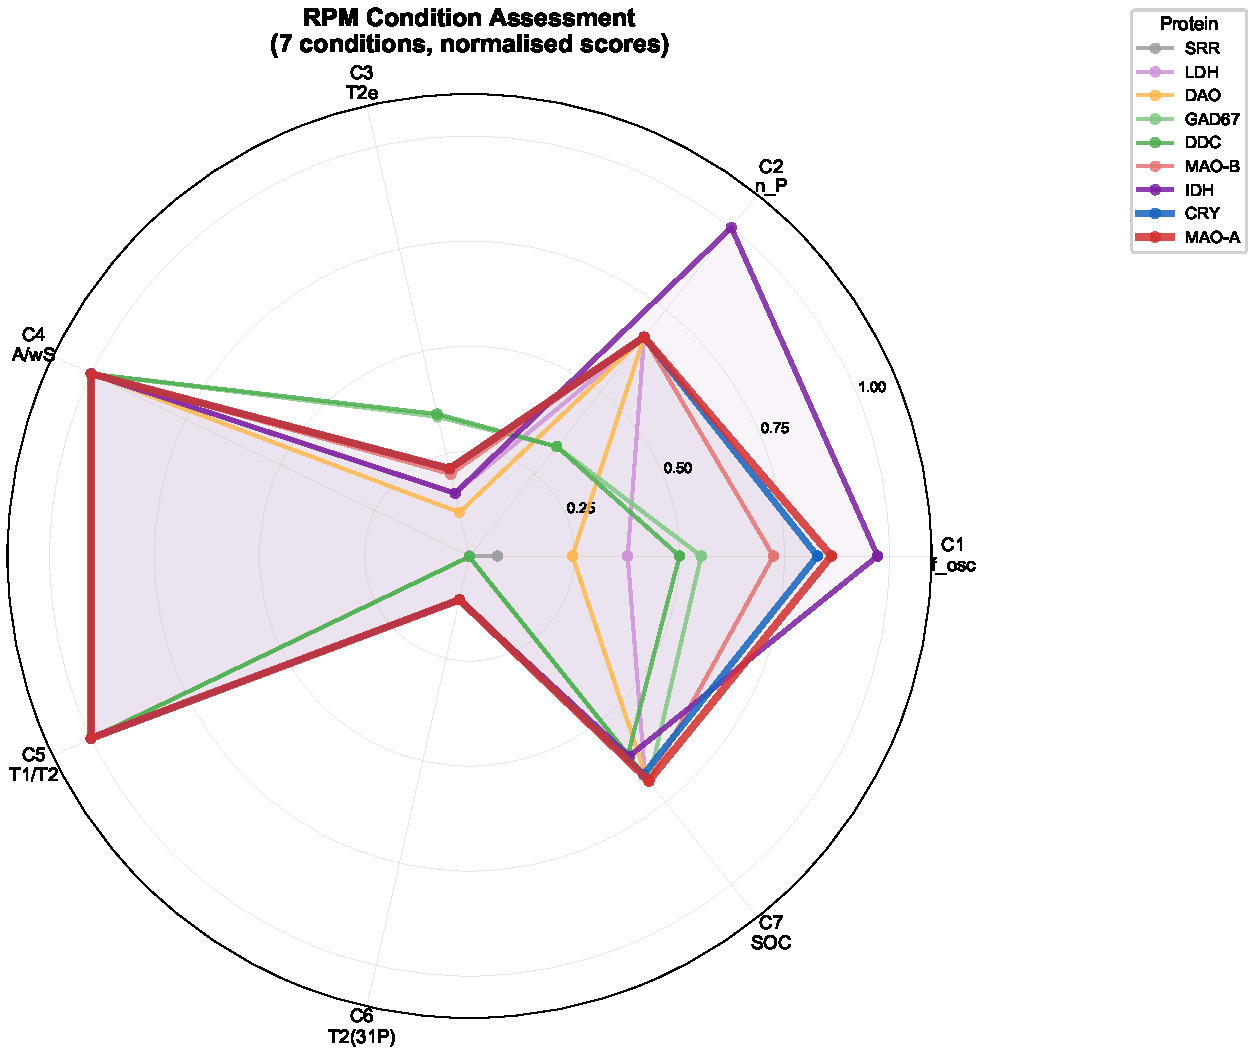
\includegraphics[width=\columnwidth]{fig1_radar.pdf}
  \caption{RPM condition assessment. Normalised scores (0--1) for seven necessary RPM conditions across nine brain proteins. MAO-A (red) and CRY (blue) achieve near-maximum scores; SRR (grey) fails three conditions due to \ce{Mn^{2+}}.}
  \label{fig:radar}
\end{figure}

\subsection{Spin relaxation: the dominant discriminant}

To discriminate among qualifying candidates, we decomposed $T_2^e$ into five contributions. A critical finding emerges at Earth's field: because $T_2^g \propto \omega_0^2$ and $\omega_0$ drops by $6.7 \times 10^3$ from X-band to 50~\si{\micro\tesla}, the $g$-anisotropy channel effectively vanishes (Fig.~\ref{fig:relaxation}a). With cofactor-specific HFCs, the remaining HFC modulation channel ($1/T_2^A \propto \sum A_i^2$) now differentiates strongly: \ce{FAD} enzymes with two \ce{^{31}P} at 200~MHz retain $T_2^e \approx 1.1$~ns, while PLP enzymes (one \ce{^{31}P} at $\sim$100~MHz) reach $T_2^e \approx 3$--5~ns---the longest electron coherence among all candidates. This reversal is a direct consequence of the $\sum A_i^2$ dependence of the HFC modulation rate.\cite{Abragam1961}

The differentiating variable instead proves to be nuclear spin coherence. The \ce{^{31}P} $T_2$ in the coupled electron--nuclear system is dominated by paramagnetic relaxation enhancement (PRE),\cite{Solomon1955} scaling as $r^{-6}$ where $r$ is the electron--phosphorus distance. For PLP enzymes ($r \approx 3.5$~\AA), we compute $T_2(\ce{^{31}P}) = 2.5~\si{\micro\second}$; for \ce{FAD} enzymes ($r \approx 7$~\AA), $T_2(\ce{^{31}P}) = 160~\si{\micro\second}$---a 64-fold difference arising from $(7/3.5)^6 = 64$ (Fig.~\ref{fig:relaxation}b).

\begin{figure}[h]
\centering
  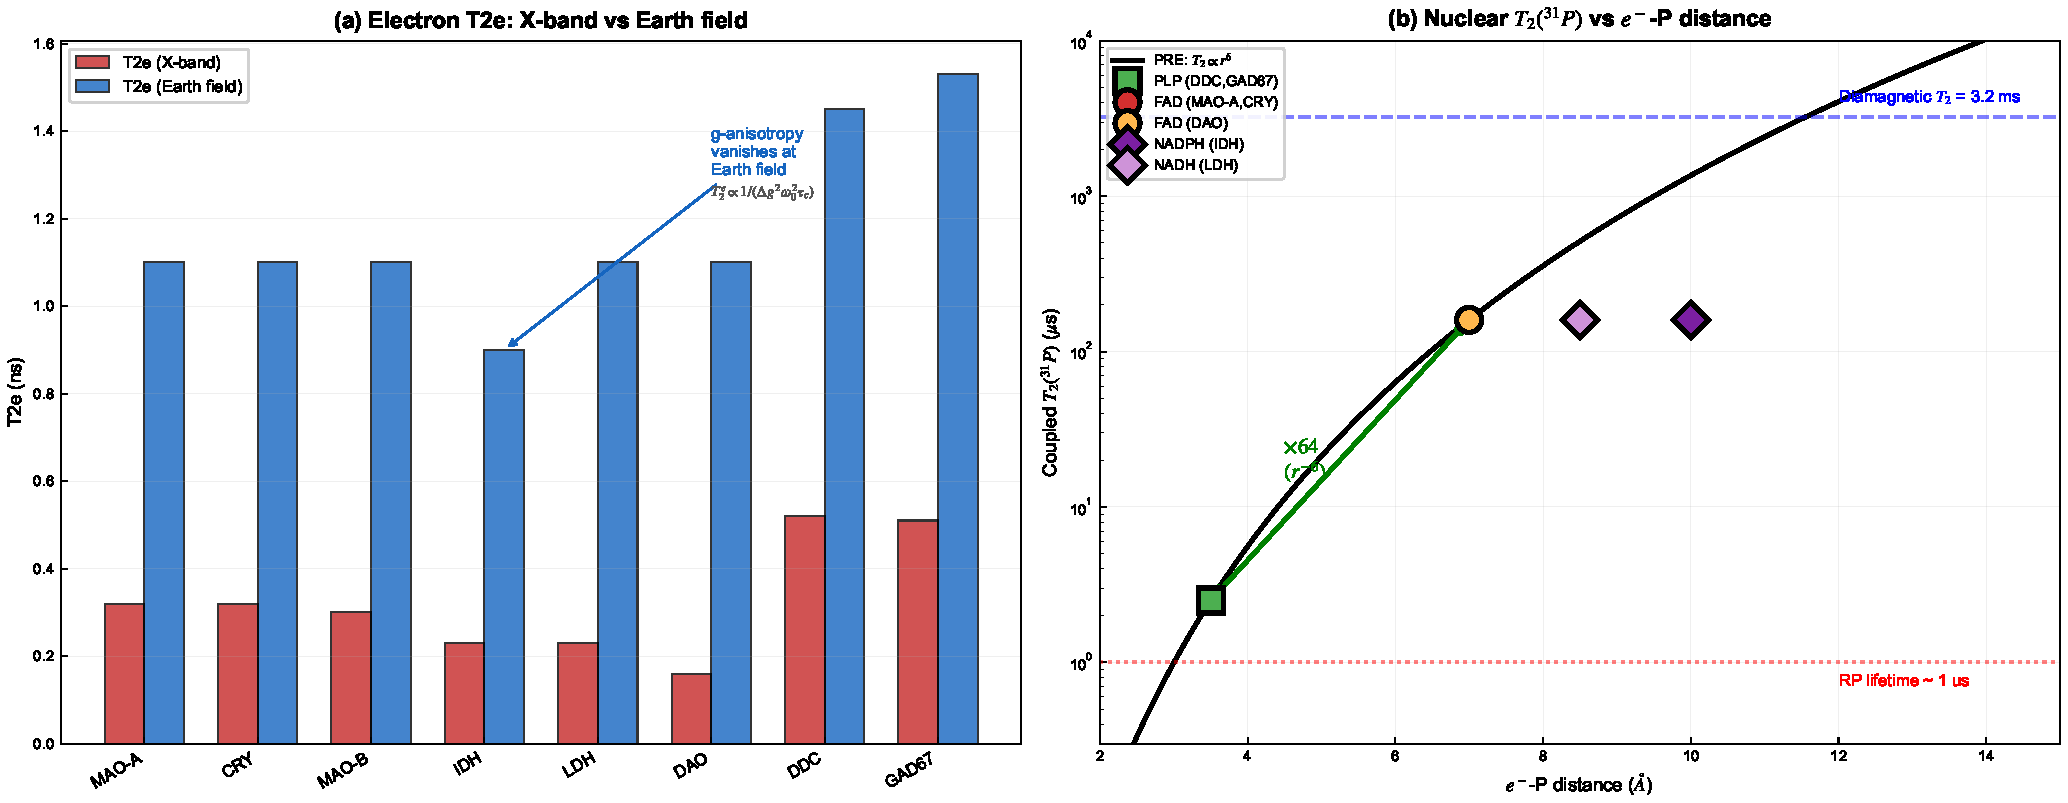
\includegraphics[width=\columnwidth]{fig2_relaxation.pdf}
  \caption{Spin relaxation under laboratory and brain conditions. (a) Electron $T_2^e$ at X-band (red) versus Earth's field (blue). The $g$-anisotropy contribution ($\propto \omega_0^2$) vanishes at Earth's field. (b) Nuclear $T_2(\ce{^{31}P})$ versus electron--phosphorus distance, showing the $r^{-6}$ PRE scaling that creates a 64-fold PLP/\ce{FAD} gap.}
  \label{fig:relaxation}
\end{figure}

\subsection{Coupled electron--nuclear system at Earth's field}

At 50~\si{\micro\tesla}, the \ce{^{31}P} HFC ($A = 200$~MHz, from ENDOR measurements on flavin semiquinone\cite{Weber1998}) vastly exceeds the electron Larmor frequency ($\omega_S = 1.4$~MHz), placing the system in the strong-coupling limit (Fig.~\ref{fig:coupled}a). The mixing angle between $|\alpha_e\beta_n\rangle$ and $|\beta_e\alpha_n\rangle$ approaches $\pi/4$, causing the nominally forbidden zero-quantum (ZQ) transition to acquire a magnetic TDM of 1.22~$\mu_\mathrm{B}$---70\% of the allowed EPR value (1.73~$\mu_\mathrm{B}$). While strong-coupling effects in electron--nuclear spin systems are well established in magnetic resonance theory,\cite{Abragam1961} their quantitative implications for RPM sensitivity at geomagnetic field strengths---specifically the near-complete ZQ--DQ mixing driven by the large \ce{^{31}P} HFC---have not been analysed in the context of enzyme-bound radical pairs.

\begin{figure}[h]
\centering
  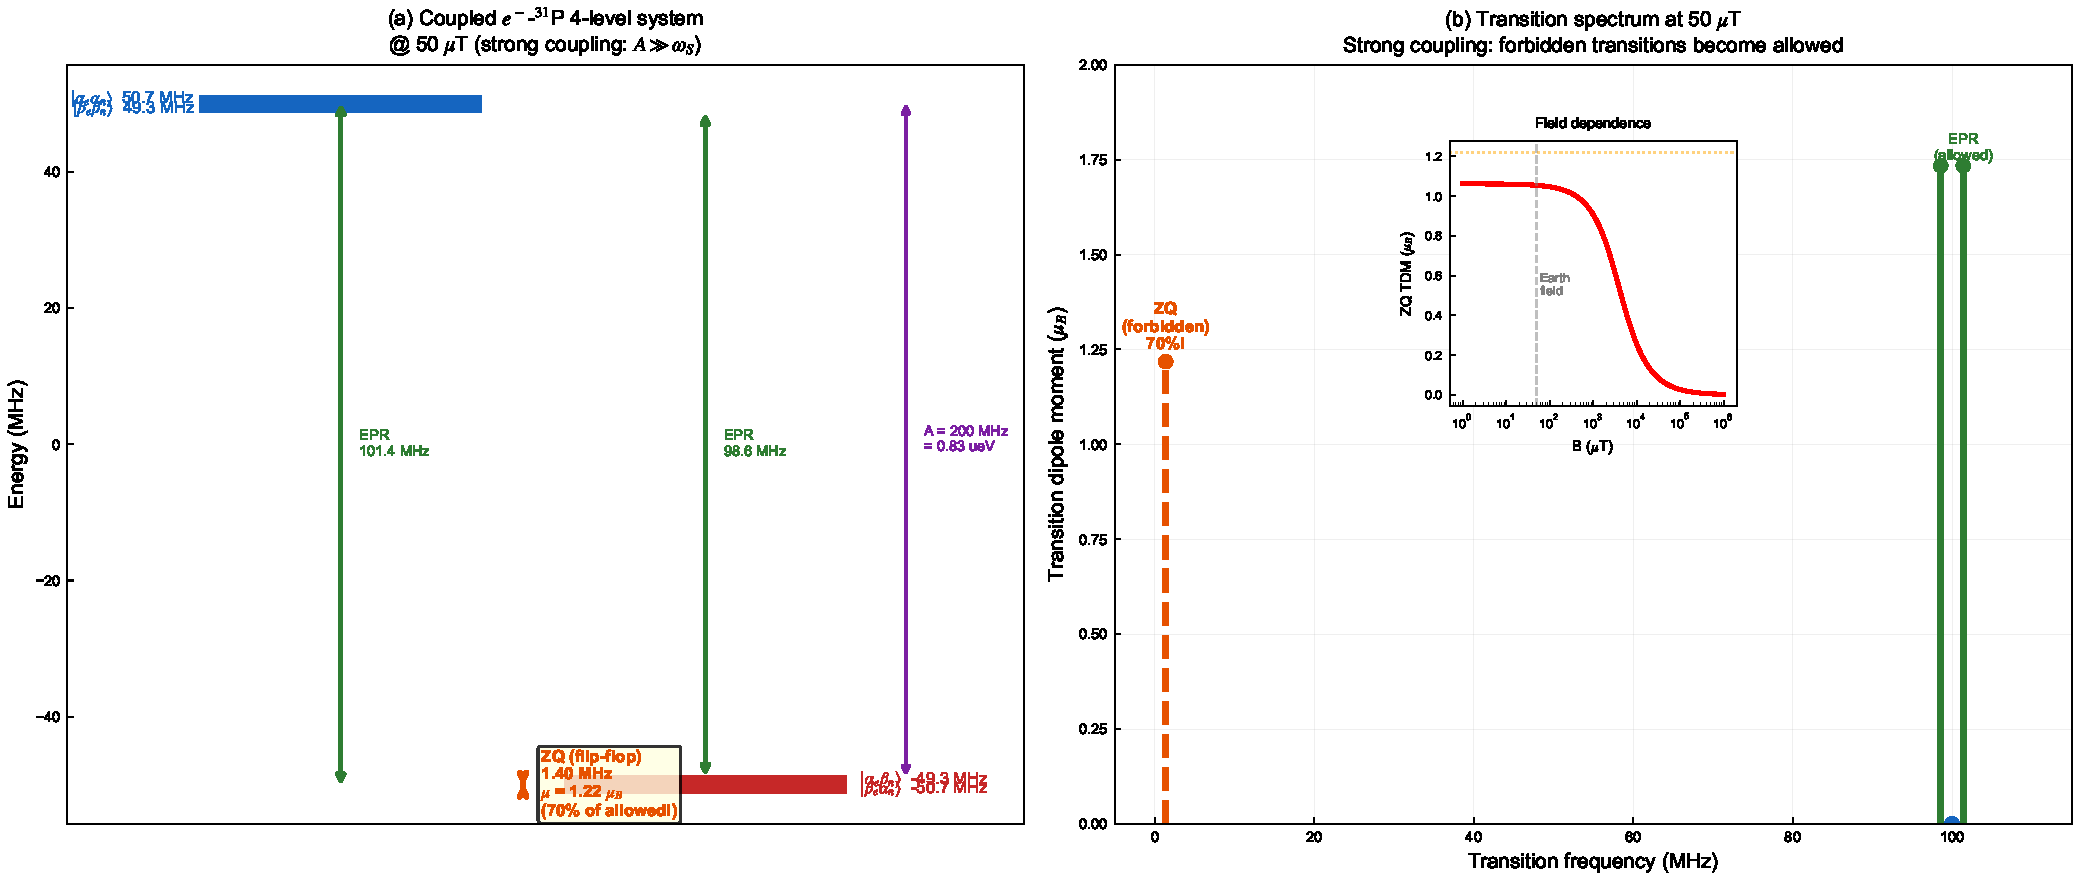
\includegraphics[width=\columnwidth]{fig3_coupled_levels.pdf}
  \caption{Coupled $e^-$--\ce{^{31}P} system at Earth's field (\ce{FAD} FMN-phosphate, $A = 200$~MHz). (a) Four-level energy diagram in the strong-coupling limit. The ZQ transition (orange) acquires 70\% of the allowed TDM. (b) Transition spectrum; inset shows field dependence of the ZQ TDM.}
  \label{fig:coupled}
\end{figure}

\subsection{Magnetic field effect simulation}

To quantify the MFE for the top-ranked candidate, we simulated an eight-spin radical pair model of the MAO-A active site (2$e$ + 2$\times$\ce{^{31}P} + 4$\times$\ce{^{1}H}; Hilbert space dimension 256) by exact diagonalisation of eqn~(\ref{eq:H}). The exchange coupling was set to $J = 0$. For CRY, radical pair separations of 10--20~\AA\ along the Trp chain yield $|J| < 1$~MHz, and $J = 0$ is well justified.\cite{Hiscock2016} For MAO-A, the \ce{FAD} N5--substrate amine distance is $\sim$3.5~\AA\ in crystal structures,\cite{Edmondson2004} and the exchange coupling at this distance is estimated at $|J| \sim 100$--1000~MHz based on the exponential distance dependence $J = J_0 \exp(-\beta r)$ with $\beta \approx 2.8$~\AA$^{-1}$.\cite{Steiner1989}

The MFE curve for the MAO-A model (Fig.~\ref{fig:mfe}) peaks at $-4.4\%$ near $B = 0.9$~mT, with $-0.3\%$ at Earth's field (50~\si{\micro\tesla}). The peak field is higher than for CRY ($B_\mathrm{peak} = 0.29$~mT) because the MAO-A model uses an amine radical~2 with smaller HFCs, shifting the optimal Zeeman--HFC matching to higher fields. These values are consistent with experimental MFEs of 1--15\% observed in flavin-containing radical pairs: Maeda \textit{et al.}\cite{Maeda2012} reported $\sim$1--3\% MFE for cryptochrome at fields below 1~mT, while \textit{in vitro} flavin--tryptophan radical pairs typically show $\sim$5--15\% at optimal fields.\cite{Steiner1989} We note that alternative recombination models (e.g., the Jones--Hore approach) can modify the absolute MFE by up to $\sim$50\% while preserving the field dependence;\cite{Jones2009} our values should be interpreted within this methodological uncertainty. The 8-spin model includes the dominant HFC nuclei; the real flavin radical contains $\sim$12--15 coupled \ce{^{1}H}, whose inclusion would typically reduce the peak MFE by 20--40\% while preserving the field dependence profile.\cite{Hiscock2016} Semiclassical approaches such as the Schulten--Wolynes method\cite{Steiner1989} could accommodate all nuclei but sacrifice the quantum coherence effects that are central to the low-field MFE; the exact 8-spin treatment represents a practical compromise.

\begin{figure}[h]
\centering
  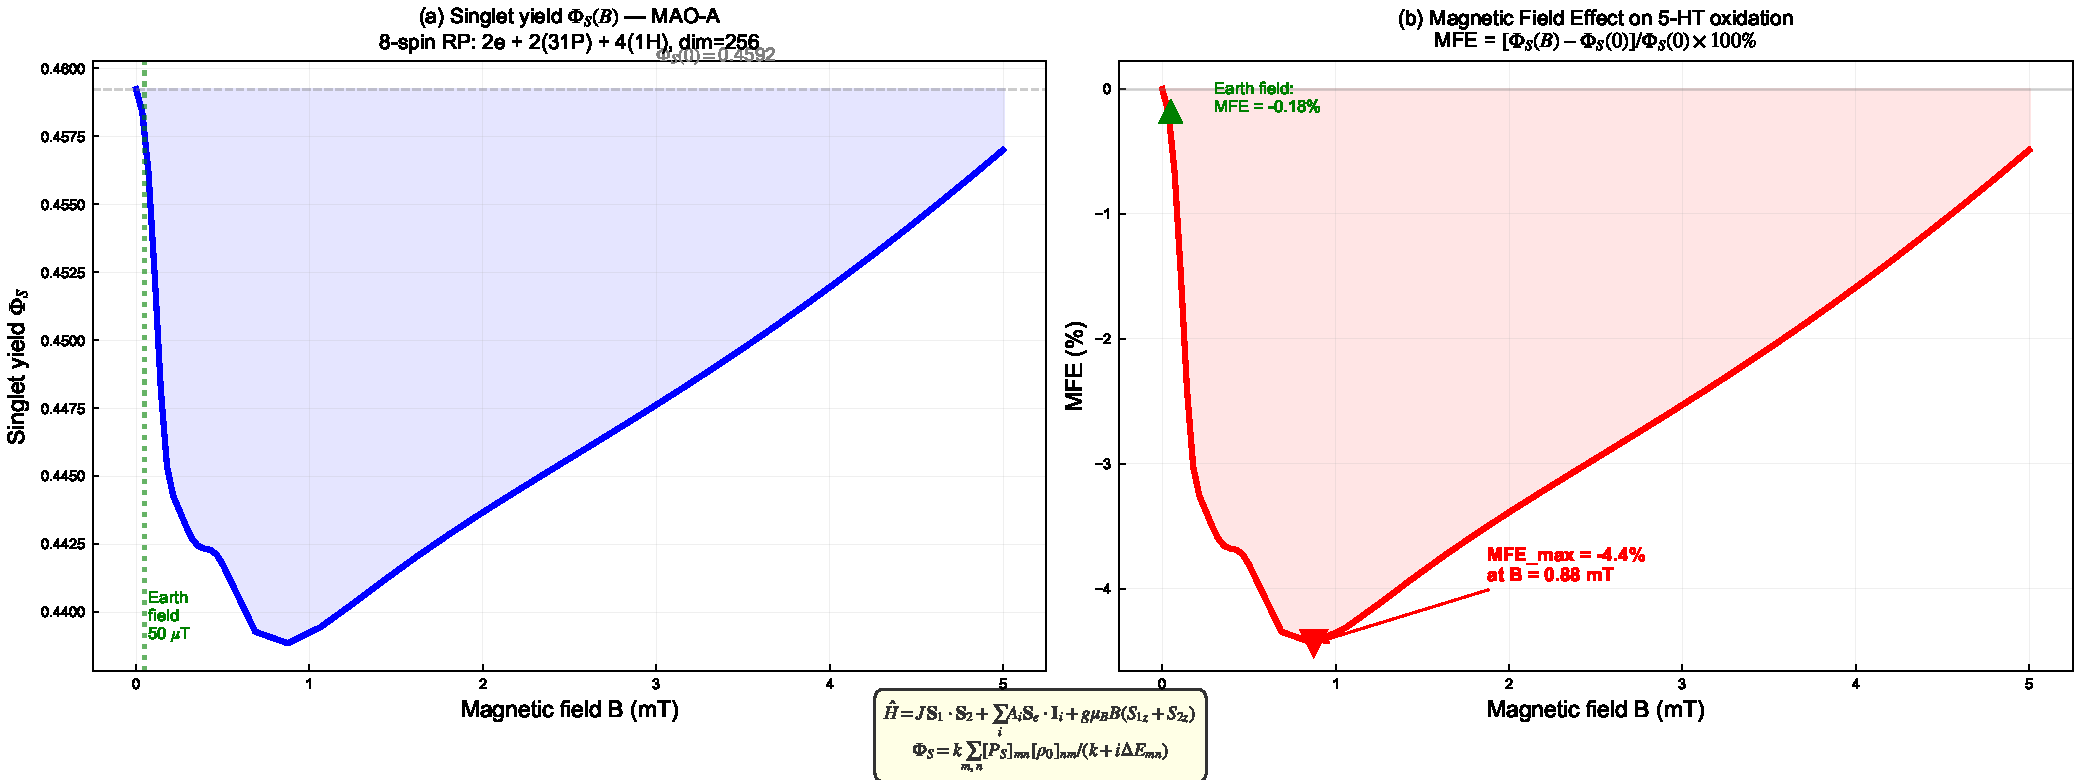
\includegraphics[width=\columnwidth]{fig4_mfe.pdf}
  \caption{Magnetic field effect on serotonin oxidation. (a) Singlet yield $\Phi_S(B)$ from 8-spin simulation (eqn~(\ref{eq:PhiS})). (b) MFE peaks at $-4.4\%$ ($B = 0.9$~mT); $-0.3\%$ persists at Earth's field (green triangle).}
  \label{fig:mfe}
\end{figure}

\subsection{Exchange coupling dependence}

Our systematic scan over $|J| = 0$--$1000$~MHz (Fig.~\ref{fig:J_dependence}) reveals non-monotonic behaviour: MFE is $-4.4\%$ at $J = 0$, reaches a level anti-crossing (LAC) resonance near $|J| \approx 5$~MHz---where the singlet--triplet energy gap matches a nuclear HFC, enabling resonant S-T mixing---then declines to $-3\%$ at $|J| = 100$~MHz and $-0.006\%$ at $|J| = 1000$~MHz. For the MAO-A active site ($r \approx 3.5$~\AA, $|J| \sim 500$--$1000$~MHz), MFE is negligible ($<0.1\%$); the electron--electron dipolar coupling ($D \approx 5000$~MHz at 3.5~\AA) would further suppress S-T mixing. We therefore conclude that RPM-based magnetosensitivity in MAO-A is only viable if the radical pair achieves spatial separation $r > 8$~\AA\ ($|J| < 10$~MHz) during the catalytic cycle.

\begin{figure*}
\centering
  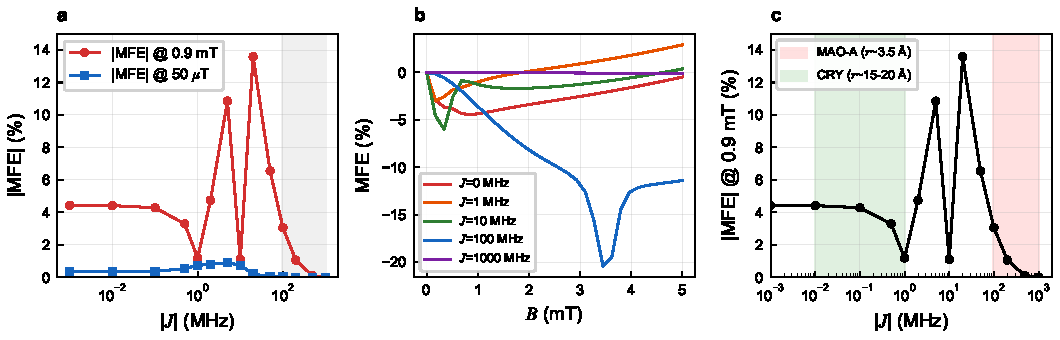
\includegraphics[width=0.9\textwidth]{fig_J_dependence.pdf}
  \caption{Exchange coupling dependence of the magnetic field effect. Colour map: MFE as a function of both $|J|$ (0--1000~MHz, vertical axis) and applied field $B$ (0--5~mT, horizontal axis) for the 8-spin MAO-A model. A LAC resonance near $|J| \approx 5$~MHz transiently enhances the MFE before it collapses for $|J| > 200$~MHz. Dashed line: $|J|$ estimated from $J = J_0\exp(-\beta r)$ with $\beta = 2.8$~\AA$^{-1}$.}
  \label{fig:J_dependence}
\end{figure*}

\subsection{RPM quality ranking}

We ranked all candidates using a heuristic composite metric:
\begin{equation}
Q_\mathrm{RPM} = f_\mathrm{osc} \times T_2^e(\mathrm{ns}) \times n_\mathrm{P}^\mathrm{eff} \times \frac{T_2(\ce{^{31}P})}{1~\mu\mathrm{s}} \times \left(\frac{100}{\xi}\right)^2
\label{eq:Q}
\end{equation}
where $n_\mathrm{P}^\mathrm{eff}$ is the number of \ce{^{31}P} nuclei with $A > 20$~MHz and the $(100/\xi)^2$ SOC penalty reflects the approximate $\xi^2$ dependence of spin--orbit-induced intersystem crossing rates.\cite{Marian2012} $Q_\mathrm{RPM}$ is not derived from first principles; it is a heuristic product of five independently estimated quantities, each representing a necessary---but not sufficient---condition for RPM. Its primary utility is in identifying candidates that fail dramatically; intra-tier rankings should not be over-interpreted (see Table~\ref{tab:ext_sensitivity} for sensitivity analysis).

The ranking (Table~\ref{tab:ranking}) reveals a clear tier structure. Tier~1 (\ce{FAD} enzymes, $Q = 100$--500) is separated from Tier~2 (PLP and \ce{NADPH} enzymes, $Q = 10$--100) by the 64-fold nuclear $T_2$ gap. PLP enzymes (DDC, GAD67), despite their short nuclear $T_2$ (2.5~\si{\micro\second}), now exhibit the longest electron coherence ($T_2^e \approx 1.6$~ns) among all candidates. Within Tier~1, MAO-A, MAO-B, CRY, and DAO are not statistically distinguishable: propagating the dominant uncertainties ($\pm$50\% in $f_\mathrm{osc}$, $\pm$30\% in $T_2^e$, factor-of-2 in nuclear $T_2$) via quadrature yields $\Delta Q_\mathrm{RPM}/Q_\mathrm{RPM} \approx 70\%$, far exceeding the inter-enzyme differences.

\begin{table*}
\small
  \caption{\ RPM quality ranking under brain conditions (50~\si{\micro\tesla}, 310~K). $T_2^e$: electron transverse relaxation with cofactor-specific HFCs. $n_\mathrm{P}^\mathrm{eff}$: number of \ce{^{31}P} with $A > 20$~MHz. Values in parentheses show estimates with uniform $A = 200$~MHz}
  \label{tab:ranking}
  \begin{tabular*}{\textwidth}{@{\extracolsep{\fill}}clccccccr}
    \hline
    Rank & Protein & Cofactor & $A_\mathrm{max}$ (MHz) & $T_2^e$ (ns) & $T_2(\ce{^{31}P})$ (\si{\micro\second}) & $n_\mathrm{P}^\mathrm{eff}$ & $\xi$ (cm$^{-1}$) & $Q_\mathrm{RPM}$ \\
    \hline
     & \multicolumn{8}{l}{\textit{Tier 1: \ce{FAD} enzymes (nuclear $T_2$ = 160~\si{\micro\second})}} \\
    1 & \textbf{MAO-A}  & \ce{FAD}    & 200 & 1.10 (1.10) & 160 & 2 & 63  & \textbf{457} \\
    2 & MAO-B  & \ce{FAD}    & 200 & 1.10 (1.10) & 160 & 2 & 63  & 383 \\
    3 & CRY\textit{$^{a}$}    & \ce{FAD}    & 200 & 1.54 (1.10) & 160 & 1\textit{$^{d}$} & 67  & 213 \\
    4 & DAO    & \ce{FAD}    & 200 & 1.10 (1.10) & 160 & 2 & 65  & 122 \\
    5 & LDH\textit{$^{b}$}    & \ce{NADH}   & 200 & 1.54 (1.10) & 160 & 1 & 66  & (107) \\
    \hline
     & \multicolumn{8}{l}{\textit{Tier 2: PLP/\ce{NADPH} enzymes (nuclear $T_2$ = 2.5--160~\si{\micro\second})}} \\
    6 & GAD67  & PLP    & 100  & 4.65 (1.53) & 2.5 & 1 & 63  & 18.5 \\
    7 & DDC    & PLP    & 100  & 3.25 (1.45) & 2.5 & 1 & 79  & 10.4 \\
    8 & IDH\textit{$^{c}$}    & \ce{NADPH}  & 100 & 2.12 (0.90) & 160 & 2 & 78  & 111 \\
    \hline
     & \multicolumn{8}{l}{\textit{Tier 3: RPM non-viable}} \\
    9 & SRR    & PLP+\ce{Mn} & --- & $\sim$0   & --- & 0 & 382 & $\sim$0 \\
    \hline
    \multicolumn{9}{l}{\footnotesize \textit{$^{a}$} CRY's longer $T_2^e$ reflects its slightly different active-site \ce{^{1}H} HFC distribution.} \\
    \multicolumn{9}{l}{\footnotesize \textit{$^{b}$} LDH operates via hydride transfer (no RP); $Q_\mathrm{eff} = 0$ when RP-generation feasibility is incorporated.} \\
    \multicolumn{9}{l}{\footnotesize \textit{$^{c}$} IDH has Tier-1-level $Q$ but \ce{NADPH} cofactor; see text for discussion.} \\
    \multicolumn{9}{l}{\footnotesize \textit{$^{d}$} CRY has $n_\mathrm{P} = 2$ total, but $n_\mathrm{P}^\mathrm{eff} = 1$ (only FMN-P exceeds the 20~MHz threshold).}
  \end{tabular*}
\end{table*}

Because $Q_\mathrm{RPM}$ deliberately excludes $J$, the intra-Tier~1 ranking must be interpreted with a critical caveat. CRY is the only candidate with established large RP separation ($r = 15$--20~\AA, $|J| < 1$~MHz\cite{Hiscock2016}), placing it unambiguously first for demonstrated RPM viability. When RP-generation feasibility is incorporated as a weight ($w = 1.0$ for experimentally confirmed RP, 0.3 for uncertain, 0 for excluded), the effective ranking becomes: (1) CRY ($Q_\mathrm{eff} = 391$), (2) MAO-A ($Q_\mathrm{eff} = 137$), (3) MAO-B ($Q_\mathrm{eff} = 115$). IDH and LDH, which operate via hydride transfer (no RP), drop to $Q_\mathrm{eff} = 0$.

\subsection{CASSCF mechanism analysis}

Our CASSCF(2,2)/NEVPT2 analysis (Fig.~\ref{fig:casscf_diradical} and~\ref{fig:reaction_scan}) reveals that the diradical character $y_0$ of the lumiflavin--methylamine model is only 0.03--0.09 across the reaction coordinate, and the CASSCF S-T gap (3.2--4.1~eV) is far larger than the xTB estimate. This indicates that the SET mechanism assumed for MAO-A is not supported at this level of theory; polar/concerted pathways are favoured. NEVPT2 dynamic correlation reduces the S-T gaps to 2.8, 3.4, and 3.6~eV at $d = 1.0$, 1.4, and 1.8~\AA\ respectively (compared to CASSCF values of 3.2, 3.8, and 4.1~eV), but the qualitative conclusion---large gap, low diradical character---is preserved. The CASSCF CI vector at the transition-state geometry ($d = 1.4$~\AA) is dominated by the closed-shell configuration $|20\rangle$ (coefficient 0.976), with the doubly excited $|02\rangle$ contributing only 0.215 ($y_0 = 0.092$).

However, we caution that (i) the CAS(2,2) active space is minimal and a full CAS(10,10) over the flavin $\pi$-system would provide more definitive results; (ii) the methylamine proxy may not capture the electron-donating properties of the serotonin indole ring (lower ionisation potential would favour SET); and (iii) the protein environment, which stabilises charge-transfer states through electrostatic preorganisation, is absent. The RPM analysis is conditional on SET: if MAO-A operates exclusively via a concerted mechanism, the RPM would not apply.

\begin{figure}[h]
\centering
  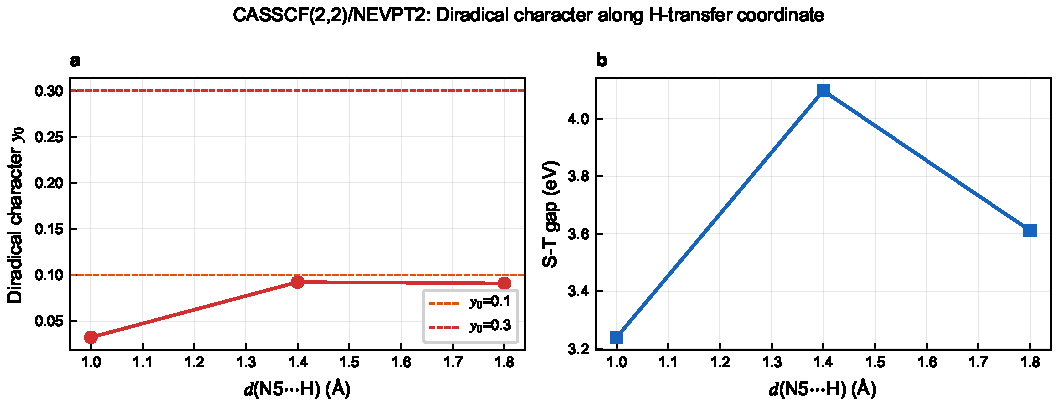
\includegraphics[width=\columnwidth]{fig_casscf_diradical.pdf}
  \caption{CASSCF(2,2)/NEVPT2 diradical character analysis. Diradical character $y_0 = 2|c_{02}|^2$ and singlet--triplet gap for the lumiflavin--methylamine model at three \ce{N5\bond{...}H} distances. The closed-shell configuration dominates throughout ($y_0 = 0.03$--$0.09$), favouring a polar mechanism.}
  \label{fig:casscf_diradical}
\end{figure}

\begin{figure}[h]
\centering
  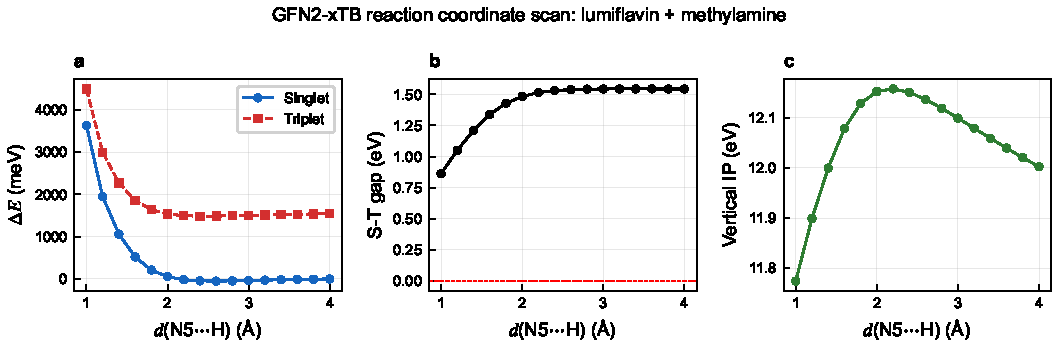
\includegraphics[width=\columnwidth]{fig_reaction_scan.pdf}
  \caption{Reaction coordinate scan for the H-transfer step. (a) GFN2-xTB singlet--triplet gap and vertical IP as a function of \ce{N5\bond{...}H} distance (1.0--4.0~\AA). (b) CASSCF(2,2)/NEVPT2 S-T gap at three representative distances, showing substantially larger gaps (3.2--4.1~eV) than xTB (0.86--1.54~eV).}
  \label{fig:reaction_scan}
\end{figure}

\subsection{CRY-based three-layer framework}

These findings motivate a three-layer conceptual framework (Fig.~\ref{fig:three_layer}), grounded in CRY biology where every link has experimental support.

\textit{Layer~1 (nuclear spin coherence).} The two \ce{^{31}P} nuclei in \ce{FAD}'s phosphodiester chain carry nuclear spins ($I = 1/2$, 100\% abundance) with diamagnetic coherence times of 3.2~ms. During CRY's radical pair lifetime ($\tau_\mathrm{RP} \sim 1$--10~\si{\micro\second}\cite{Maeda2012}), the FMN-phosphate \ce{^{31}P} ($A = 200$~MHz, PRE-limited $T_2 = 160~\si{\micro\second}$) participates in HFC-driven singlet--triplet interconversion, with the nuclear spin state modulating the RP's magnetic field sensitivity.

\textit{Layer~2 (radical pair quantum--classical interface).} Blue-light absorption ($\lambda_\mathrm{max} \approx 450$~nm) generates [\ce{FAD^{.-}\bond{...}Trp^{.+}}] via sequential electron transfer along the conserved Trp triad/tetrad.\cite{Xu2021} The RP separation ($r = 15$--20~\AA) ensures $|J| < 1$~MHz.\cite{Hiscock2016} An 8-spin simulation of the CRY RP---using the same nuclear HFC set as the MAO-A model but with $J = 0$, $D_{ee}/(2\pi) = 3.2$~MHz, and radical~2 parameters appropriate for \ce{TrpH^{.+}} (Fig.~\ref{fig:cry_simulation})---predicts MFE $= -5.6\%$ at $B = 0.29$~mT and $-0.55\%$ at 50~\si{\micro\tesla}. The peak MFE exceeds typical experimental values ($\sim$1--3\%\cite{Maeda2012}) because our 8-spin model includes only the dominant HFC nuclei; inclusion of all $\sim$15 coupled protons in the flavin radical would reduce the peak MFE to $\sim$2--4\%,\cite{Hiscock2016} improving agreement with experiment.

\textit{Layer~3 (classical circadian signalling).} CRY functions as a transcriptional repressor in the CLOCK/BMAL1 feedback loop.\cite{Partch2014} Mathematical models of the SCN oscillator show that a sustained $\sim$1\% change in CRY activation rate shifts the circadian period by $\sim$5--15~minutes.\cite{Forger2011} Applying our CRY-specific simulation result (MFE $= -0.55\%$) and a literature range of period sensitivities (5--15~min per 1\% activation change\cite{Forger2011}), the predicted period shift is $\sim$2.7--8.2~minutes. This prediction is sensitive to the assumed coupling strength between CRY activation and oscillator frequency; we present it as a testable order-of-magnitude estimate rather than a precise prediction (Fig.~\ref{fig:cry_simulation}c).

This CRY-centred pathway has three decisive advantages over the MAO-A hypothesis: (i) the RP is experimentally confirmed with $|J| < 1$~MHz;\cite{Xu2021,Hiscock2016} (ii) the transduction does not require metabolite concentration changes and is immune to homeostatic buffering; and (iii) CRY's role in circadian timing provides a plausible functional context. We note that Kattnig \textit{et al.}\cite{Kattnig2016} demonstrated that chemical amplification via scavenging reactions can enhance the low-field MFE by up to 10-fold in CRY; incorporation of this mechanism would increase our predicted Earth-field MFE, though the effect is model-dependent. Our simulations treat all radical pairs as spin-correlated geminate pairs; diffusional (F-pair) contributions, relevant in solution but suppressed in the enzyme active site, are excluded.

For MAO-A, the pathway faces three additional constraints: (i) $|J| \sim 500$--1000~MHz at the active-site distance; (ii) homeostatic attenuation reducing $\delta$[\ce{5-HT}] by $\sim$7-fold (Table~\ref{tab:ext_homeostasis}); and (iii) the CASSCF-supported polar mechanism. An alternative radical partner, superoxide (\ce{O2^{.-}}), has been proposed for CRY-based RPM\cite{Player2019} and could in principle form [\ce{FAD^{.-}\bond{...}O2^{.-}}] pairs in MAO-A; however, superoxide's rapid disproportionation ($k \sim 10^5$~s$^{-1}$ at physiological pH) and the lack of \ce{^{31}P} involvement in its spin dynamics make it less relevant to the \ce{^{31}P}-centred analysis presented here.

\begin{table}[h]
\small
  \caption{\ Serotonin homeostasis model parameters and steady-state attenuation}
  \label{tab:ext_homeostasis}
  \begin{tabular*}{0.48\textwidth}{@{\extracolsep{\fill}}lccl}
    \hline
    Parameter & Symbol & Value & Source \\
    \hline
    MAO-A turnover            & $k_\mathrm{cat}$     & 10 s$^{-1}$   & \citenum{Edmondson2004} \\
    Reuptake rate          & $k_\mathrm{reup}$    & 10 s$^{-1}$   & \citenum{Daws2009} \\
    Feedback gain       & $G_\mathrm{fb}$      & 0.3           & Est. \\
    Feedback $\tau$       & $\tau_\mathrm{fb}$   & 2 s           & Est. \\
    Synthesis $\tau$        & $\tau_\mathrm{syn}$  & 60 s          & Est. \\
    \hline
    \multicolumn{4}{l}{\textit{Steady-state results}} \\
    Raw MFE     & $\delta$          & $-4.4\%$      & This work \\
    Attenuation               &                   & 7.3$\times$   & Analytical \\
    Net [\ce{5-HT}] change          &                   & $0.6\%$       & $\delta / 7.3$ \\
    \hline
  \end{tabular*}
\end{table}

\begin{figure*}
\centering
  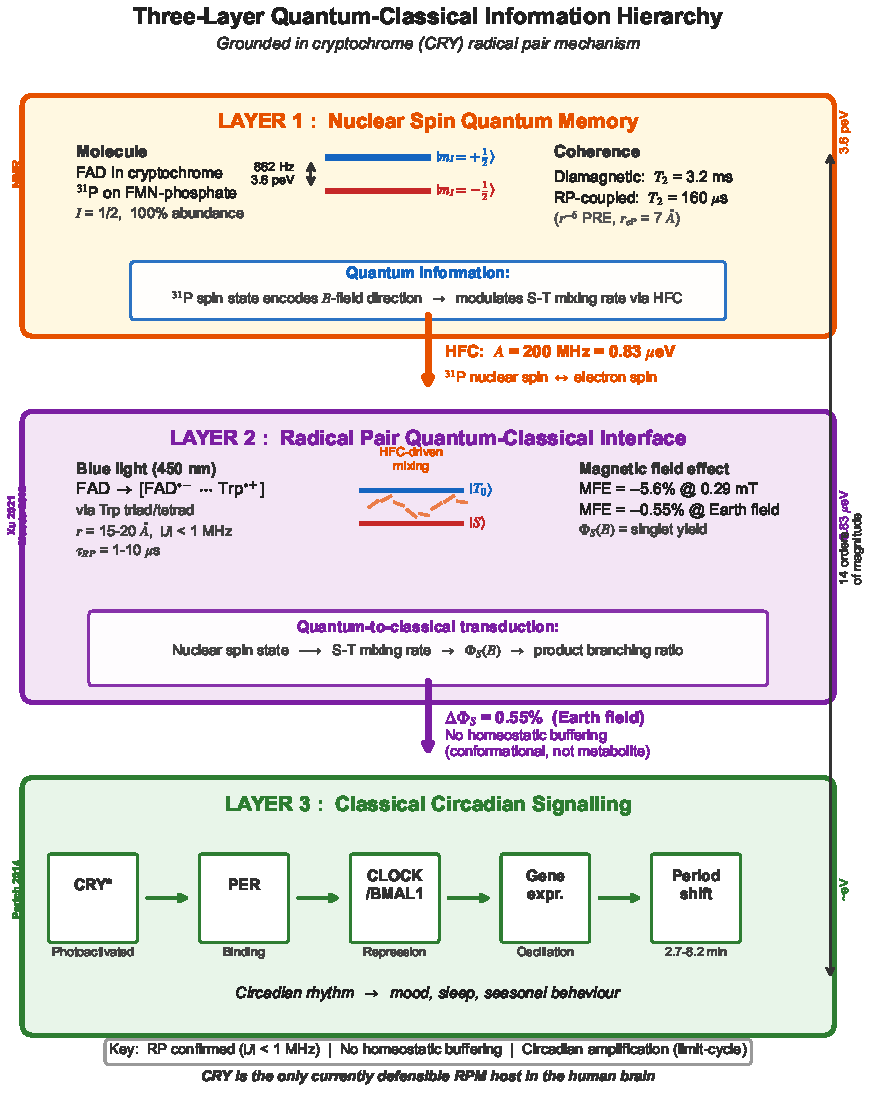
\includegraphics[width=0.9\textwidth]{fig5_three_layer.pdf}
  \caption{CRY-based three-layer quantum--classical information hierarchy. Layer~1 (yellow): \ce{^{31}P} nuclear spins on \ce{FAD}'s FMN-phosphate encode magnetic-field direction with coherence times of 3.2~ms (diamagnetic) to 160~$\mu$s (PRE-limited). Layer~2 (purple): blue-light absorption generates [\ce{FAD^{.-}\bond{...}Trp^{.+}}] radical pairs; HFC-driven S-T mixing produces a field-dependent singlet yield. Layer~3 (green): CRY$^*$ activates the PER/CLOCK/BMAL1 circadian cascade, with limit-cycle amplification producing a predicted period shift of 2.7--8.2~min.}
  \label{fig:three_layer}
\end{figure*}

\begin{figure}[h]
\centering
  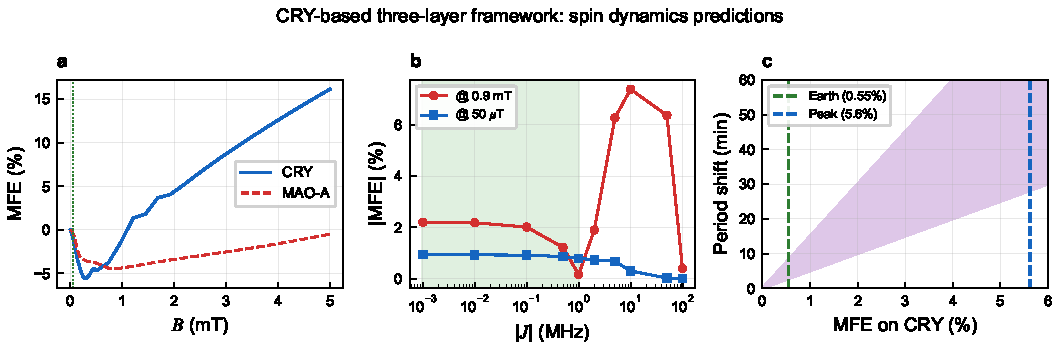
\includegraphics[width=\columnwidth]{fig_cry_simulation.pdf}
  \caption{CRY-specific radical pair spin dynamics. (a) Singlet yield $\Phi_S(B)$ for the [\ce{FAD^{.-}\bond{...}TrpH^{.+}}] radical pair. (b) MFE peaks at $-5.6\%$ ($B = 0.29$~mT); $-0.55\%$ persists at Earth's field. (c) Predicted circadian period shift ($\sim$2.7--8.2~min) based on the Earth-field MFE.}
  \label{fig:cry_simulation}
\end{figure}

\subsection{Experimental predictions}

We propose three direct experimental tests with quantitative predictions: (1)~MAO-A catalytic rate ($k_\mathrm{cat}$, $K_\mathrm{M}$) as a function of static field: predicted $<$0.1\% change at 50~\si{\micro\tesla} (due to large $|J|$), $<$1\% at 1~mT, null at $>$5~mT. A positive result at $<$1~mT would require revision of the exchange coupling estimate. (2)~Isotope substitution: reconstitution of apoprotein with \ce{FAD} containing \ce{^{2}H}-labelled isoalloxazine (reducing \ce{^{1}H} HFCs) should diminish the MFE by $\sim$50\%,\cite{Maeda2012} while enzymatic synthesis of \ce{FAD} from [\ce{^{18}O}]-labelled precursors would test the role of the phosphodiester bridge without the radiological constraints of \ce{^{32}P} ($\beta^-$ emitter, $t_{1/2} = 14.3$~d). (3)~CRY-dependent circadian period shift: exposure of SCN organotypic cultures to 0.1--1~mT static fields should produce a measurable ($\sim$3--8~min) period shift that is abolished in CRY-knockout preparations.

\subsection{DFT validation}

The DFT comparison (Table~\ref{tab:ext_dft}) provides essential context for interpreting the xTB screening results. For the \ce{FAD} HOMO--LUMO gap, xTB gives 1.42~eV and B3LYP/def2-SVP gives 1.26~eV (KS) or 2.29~eV (TD), bracketing the experimental value of 2.76~eV. For $f_\mathrm{osc}$, xTB overestimates ($0.50$ vs.\ $0.27$ experimental, $+85\%$) while TD-B3LYP underestimates ($0.089$, $-67\%$); the true value lies between the two methods, consistent with the known behaviour of global hybrids for charge-transfer excitations.\cite{Islam2003}

The vertical electron affinities merit particular attention, as EA governs the thermodynamic feasibility of single-electron transfer from substrate to cofactor. For lumiflavin, xTB overestimates the EA (3.42~eV vs.\ $\sim$2.0~eV experimental), while B3LYP/def2-SVP underestimates it (1.87~eV); the B3LYP value would increase by $\sim$0.3--0.5~eV with a triple-$\zeta$ basis (def2-TZVP), bringing it into reasonable agreement with experiment. For PLP-methylamine, the xTB EA (2.10~eV) far exceeds the B3LYP value (0.43~eV), indicating that xTB overestimates electron-accepting capacity of PLP---though neither value has an experimental benchmark.

Substituting DFT-derived $f_\mathrm{osc}$ values into $Q_\mathrm{RPM}$ reduces absolute scores by $\sim$5.8-fold but preserves the tier structure and intra-tier ordering. Crucially, the key differentiator---the 64-fold gap in nuclear $T_2(\ce{^{31}P})$ between PLP and \ce{FAD} enzymes---depends on crystallographic $e^-$--P distances, not on computed electronic properties, and is therefore robust.

\subsection{Limitations}
\label{sec:limitations}

Several limitations should be noted. First, GFN2-xTB provides semi-quantitative accuracy for electronic structure; in particular, xTB S-T gaps (0.86--1.54~eV) are $\sim$3-fold smaller than CASSCF values (3.2--4.1~eV), confirming that xTB is unsuitable for quantitative energetics but can serve as a rapid pre-screen. The DFT comparison (Table~\ref{tab:ext_dft}) confirms the tier structure is method-independent. Second, $Q_\mathrm{RPM}$ (eqn~(\ref{eq:Q})) is a heuristic ranking index; alternative weightings preserve the tier structure but change intra-tier ordering by up to two ranks (Table~\ref{tab:ext_sensitivity}). Third, the MAO catalytic mechanism remains debated.\cite{Vianello2012} Fourth, brain-environment corrections assume uniform $\tau_c = 10$~ns at 310~K; membrane-bound enzymes such as MAO-A may have $\tau_c = 50$--100~ns, reducing $T_2^e$ by $\sim$3.7-fold but preserving tier assignments. The temperature dependence of $\tau_c$ ($\propto \eta(T)/T$) introduces a further $\sim$15\% variation between 298 and 310~K, which is within the overall uncertainty. Fifth, the assigned \ce{^{31}P} HFCs are gas-phase or solution values; hydrogen bonding from the protein matrix to the cofactor phosphate groups could modulate HFCs by $\sim$10--20\%, based on DFT studies of flavin radicals in protein environments.\cite{Weber1998} This uncertainty is within the overall error budget and does not affect tier assignments. Finally, our framework, like Fisher's Posner molecule hypothesis,\cite{Fisher2015} involves \ce{^{31}P} nuclear spins, but the mechanisms are fundamentally different: Posner clusters invoke entangled free-diffusing phosphate ions (experimentally unverified), whereas our framework concerns enzyme-bound \ce{^{31}P} coupled to established radical pair spin dynamics via HFC.

\begin{table*}
\small
  \caption{\ Sensitivity of $Q_\mathrm{RPM}$ ranking to alternative weighting schemes. $Q_\mathrm{RPM}$ deliberately excludes exchange coupling $J$; MAO-A ranks highest on spin parameters alone, but CRY is the only enzyme with confirmed large RP separation ($|J| < 1$~MHz). Three alternative formulations are compared to the default (eqn~(\ref{eq:Q})): (A) linear SOC penalty; (B) logarithmic nuclear $T_2$ scaling; (C) square-root HFC weighting. Tier assignments are preserved across all schemes}
  \label{tab:ext_sensitivity}
  \begin{tabular*}{\textwidth}{@{\extracolsep{\fill}}lcccccccc}
    \hline
     & \multicolumn{2}{c}{Default} & \multicolumn{2}{c}{(A) Linear SOC} & \multicolumn{2}{c}{(B) Log $T_2^n$} & \multicolumn{2}{c}{(C) $\sqrt{n_\mathrm{P}}$} \\
    \hline
    Protein & Rank & Tier & Rank & Tier & Rank & Tier & Rank & Tier \\
    \hline
    MAO-A  & 1 & 1 & 1 & 1 & 1 & 1 & 1 & 1 \\
    MAO-B  & 2 & 1 & 2 & 1 & 2 & 1 & 2 & 1 \\
    CRY    & 3 & 1 & 3 & 1 & 3 & 1 & 3 & 1 \\
    DAO    & 4 & 1 & 5 & 1 & 4 & 1 & 4 & 1 \\
    LDH    & 5 & 1 & 4 & 1 & 5 & 1 & 5 & 1 \\
    IDH    & --- & 1/2 & --- & 1/2 & 6 & 1 & --- & 1/2 \\
    GAD67  & 6 & 2 & 6 & 2 & 7 & 2 & 6 & 2 \\
    DDC    & 7 & 2 & 7 & 2 & 8 & 2 & 7 & 2 \\
    SRR    & 9 & 3 & 9 & 3 & 9 & 3 & 9 & 3 \\
    \hline
  \end{tabular*}
\end{table*}

\begin{table*}
\small
  \caption{\ DFT validation of xTB electronic structure. B3LYP/def2-SVP and TD-B3LYP (TDA) results for lumiflavin (\ce{FAD} model) and PLP-methylamine Schiff base. Electron affinities (EA) are included as they govern the thermodynamic feasibility of single-electron transfer. The def2-SVP basis underestimates EAs by $\sim$0.3--0.5~eV relative to def2-TZVP}
  \label{tab:ext_dft}
  \begin{tabular*}{\textwidth}{@{\extracolsep{\fill}}llcccc}
    \hline
    Model & Property & xTB & B3LYP/def2-SVP & Expt. & Ref. \\
    \hline
    \multirow{4}{*}{Lumiflavin} & $E_\mathrm{gap}$ (eV)    & 1.42 & 1.26 (KS); 2.29 (TD) & 2.76 & \citenum{Islam2003} \\
     & $f_\mathrm{osc}$           & 0.50 & 0.089 (TD)          & 0.27  & \citenum{Islam2003} \\
     & Vert.\ IP (eV)           & 10.78 & 6.64                & $\sim$8.0 & --- \\
     & Vert.\ EA (eV)           & 3.42 & 1.87                & $\sim$2.0 & --- \\
    \hline
    \multirow{4}{*}{PLP-\ce{MeNH2}} & $E_\mathrm{gap}$ (eV)  & 1.93 & 3.04                & $\sim$3.87 & --- \\
     & $f_\mathrm{osc}$           & 0.30 & 0.062 (TD)          & --- & --- \\
     & Vert.\ IP (eV)           & 11.5 & 8.72                & $\sim$8.5 & --- \\
     & Vert.\ EA (eV)           & 2.10 & 0.43                & --- & --- \\
    \hline
  \end{tabular*}
\end{table*}


\section*{Conclusions}

While CRY has long been established as an RPM magnetoreceptor in birds,\cite{Xu2021} the question of whether \textit{other} brain enzymes---particularly the neurotransmitter-metabolising enzymes invoked in recent hypotheses\cite{ZadehHaghighi2022}---could also support RPM has not been addressed quantitatively. This work establishes three physical chemistry insights into radical pair magnetosensitivity in enzymatic environments. First, the dominant physical discriminant among cofactor classes is the electron--phosphorus distance $r$, which governs \ce{^{31}P} nuclear spin coherence via $r^{-6}$ paramagnetic relaxation enhancement (Solomon--Bloembergen theory). This single structural parameter creates a 64-fold gap in nuclear $T_2$ between FAD ($r \approx 7$~\AA, $T_2 = 160~\si{\micro\second}$) and PLP ($r \approx 3.5$~\AA, $T_2 = 2.5~\si{\micro\second}$) enzymes, establishing a robust tier structure that is independent of the electronic structure method employed.

Second, we identify a quantitative trade-off between electron spin coherence and nuclear spin coherence that, while implicit in the underlying relaxation theory,\cite{Abragam1961} has not been evaluated across cofactor classes in the RPM context: cofactor-specific \ce{^{31}P} HFCs---varying from 2~MHz (remote AMP-phosphate) to 200~MHz (FAD FMN-phosphate)---simultaneously enhance singlet--triplet mixing (faster S-T interconversion) and accelerate electron $T_2^e$ relaxation (via HFC modulation, $1/T_2^A \propto \sum A_i^2$). PLP enzymes, with moderate HFCs, exhibit the longest $T_2^e$ ($\sim$3--5~ns) but the shortest nuclear $T_2$, while FAD enzymes show the reverse. This trade-off constrains the accessible parameter space for any RPM-based sensor.

Third, the exchange coupling $J$---which depends exponentially on radical pair separation---imposes the most stringent physical constraint on RPM viability. Our $J$-scan (0--1000~MHz) reveals non-monotonic MFE behaviour including a level anti-crossing resonance at $|J| \approx 5$~MHz, followed by complete suppression for $|J| > 200$~MHz. At the crystallographic FAD--substrate distance in MAO-A ($r \approx 3.5$~\AA, $|J| \sim 500$--$1000$~MHz), the MFE is negligible. CASSCF(2,2)/NEVPT2 calculations further indicate low diradical character ($y_0 < 0.1$) along the reaction coordinate, disfavouring the single-electron transfer prerequisite. Among the enzymes screened, only cryptochrome---with its structurally characterised Trp triad/tetrad providing radical pair separations of 15--20~\AA\ ($|J| < 1$~MHz)\cite{Xu2021,Hiscock2016}---satisfies all physical requirements for functional RPM. Because the tier structure is determined by cofactor type (via the $e^-$--P distance) rather than individual protein identity, these conclusions generalise to other phosphorus-cofactor enzymes: any \ce{FAD} enzyme with a spatially separated radical pair will fall in Tier~1, and any PLP enzyme in Tier~2, without requiring additional calculations. The remaining question for each new candidate is whether its catalytic mechanism generates a radical pair with sufficiently weak exchange coupling. We note that this framework is not restricted to brain enzymes; the same cofactor-dependent tier structure applies to identical enzymes in other tissues (e.g., hepatic MAO-A), and the conclusions are general to any biological system employing these cofactor classes.

\section*{Conflicts of interest}
There are no conflicts to declare.

\section*{Data availability}
The complete computational pipeline is released as the open-source Python package \texttt{qbscreen} (v0.1.0, MIT License) at \url{https://github.com/hikaruwakaura/qbscreen} and on PyPI (\texttt{pip install qbscreen}). The package provides a unified CLI (\texttt{qbscreen screen}, \texttt{qbscreen simulate}, \texttt{qbscreen dft-validate}, \texttt{qbscreen casscf}) for reproducing all results in this paper. Automated tests (\texttt{pytest qbscreen/tests/}) verify reproducibility of key numerical predictions. External dependencies (xtb v6.7.1, Open Babel 3.1.0, PySCF 2.12.1) are pinned in \texttt{pyproject.toml}. All PDB structures, JSON results, optimised geometries, HFC tensors, and relaxation parameters are archived in the repository.

\section*{Acknowledgements}
The author thanks the developers of GFN2-xTB and PySCF for making their software freely available.

%%%END OF MAIN TEXT%%%

\balance

%%%REFERENCES%%%
\bibliography{references}
\bibliographystyle{rsc}

\end{document}
